\section{Introduction}
\label{sec:usbe_lung_introduction}
\subsection{Introduce the problem motivation and objective of study}
Interactions between mechanical waves and fluid-fluid interfaces is a
topic of interest in a variety of areas within the fluids and acoustic
communities. Shock-accelerated interest have been of particular
interest due to their applications in fusion energy and astrophysics,
and have been studied extensively \citep{Drake2005}.

While shocks are discontinuous and exhibit highly nonlinear behavior,
acoustic waves, in contrast, tend to be continuous and significantly
less non-linear. For most applications of practical interest the
behavior of acoustic waves is well captured by the acoustic wave
equation, which can be derived from linearized Euler Equations of
inviscid fluid motion. The behavior of an acoustic wave passing from
one medium to another is generally well understood to produce separate
transmitted and reflected wave, the amplitude, phase, and direction of
each depending on the material properties of the two media and the
geometry of the surface. For most practical interests fluid-solid
interfaces are unchanged by the interaction with the acoustic
waves. The same is not necessarily true for fluid-fluid
interfaces. One notable example of this is acoustic cavitation, in
which acoustic waves excite tiny gas bubble cavitation nuclei, causing
them to grow and sometimes collapse violently. This phenomena has been
researched extensively in a variety of contexts including as a
mechanism for \ac{US} bioeffects. This work is motivated to
investigate another \ac{US} bioeffects problem that also involves
acoustic waves interacting strongly with a fluid-fluid
interface. Specifically, we are interested in the behavior of alveoli,
tiny air sacs in the lung, exposed to \ac{DUS} pulses, as it has been
previously shown that \ac{DUS} can induce \ac{LH} in mammals.

Pulsed \ac{US} was first observed to cause \ac{LH} in mice over twenty
years ago, though the underlying physical damage mechanism is still
unknown \citep{Dalecki2004,OBrien2007}.

DUS-induced lung hemorrhage has been shown to be non-thermal in nature
\citep{Dalecki2004} though appears not be caused by
cavitation. Currently We use computation and theory to investigate
interactions between acoustic waves and fluid-fluid interfaces. In
particular we demonstrate that, like shocks, acoustic waves are
capable of depositing vorticity at interfaces and that, this vorticity
is capable of growing interface perturbations in a predicable
manner. We go on to discuss the relevance of our results to
DUS-induced \ac{LH}.


\subsection*{Background}
While the problem of acoustic waves interacting with fluid-fluid
interfaces in the lungs does not appear to have been previously
studied in the present context, there has been much past work in both
areas separately that provides context for this study and direction to
our efforts. Below we attempt to summarize the relevant research in
each area, as it relates to the present work.

\subsubsection*{background on waves}

\subsubsection*{background on DUS-induced \ac{LH}}
From an acoustics standpoint the majority of prior analysis begins
from the linearized Euler equations of fluid motion. As such, it is
not surprising that acoustically generated baroclinic vorticity at
interfaces has not been previously considered as a potential mechanism
for DUS-induced lung hemorrhage, as this is an entirely nonlinear
effect that only becomes important due to he sharp density gradients
that exist in the lungs between air and surrounding tissues and
fluids.






% Medical \ac{US}, while remaining
% acoustic in nature, often features nonlinear pressure waveforms. This
% is a result of the mechanisms used to generate the waves and MPa order
% differences between high- and low-pressure regions of the wave,
% causing strong variations in sound speed within the wave, leading to
% wave steepening and deformation. Up to this point, there is still
% little research investigating the nonlinear contributions to
% interactions between acoustic waves and fluid-fluid interfaces.

% One problem that nonlinear acoustic effects may be of particular
% relevance to is Diagnostic \Ac{US} (DUS)-induced Lung Hemorrhage
% (\ac{LH}).  Lung \ac{DUS} has become increasingly common in critical care
% situations (Lichtenstein, 2009), and \ac{LH} is the only bioeffect of
% non-contrast diagnostic \ac{US} known to occur in mammals.
% Presently the damage mechanisms underlying \ac{DUS}-induced \ac{LH} are unknown.
% And while it does not appear to be a clinical medical problem of
% significant concern, it is one that we must understand if we hope to
% improve lung \ac{DUS} by expanding the US regimes used in clinical
% application. This work aims to investigate nonlinear fluid effects,
% specifically baroclinic torque at tissue-air interfaces in the lungs,
% as a possible damage mechanism of \ac{DUS}-induced lung hemorrhage. To
% accomplish this investigation we will perform numerical simulations of
% relevant wave-interface interactions and leverage the analytical tools
% commonly used in the fluids community to analyze shock-interface
% interactions.  The problem of US-induced lung hemorrhage is not a new
% problem.  It was first discovered in mice exposed to a lithotripter
% pulse (Child et al., 1990), and much work has been since performed to
% study it more deeply. Previous research has primarily aimed at three
% specific ends: (1) Determining the dependence of damage
% characteristics and thresholds on the subject; (2) Determining the
% dependence of damage characteristics and thresholds on the US
% properties; and (3) Investigating the damage mechanism by which the
% hemorrhage occurs.  While our work is fundamental in nature aims to
% contribute to the third area and proposes US-induced circulation
% deposition in the lungs as a potential mechanism for \ac{DUS}-induced
% hemorrhage. Furthermore, in pursuing this investigation we will be
% studying wave-interface interactions for acoustic waves of varying
% shape, frequency content, and amplitude, and plan to compare our
% results for deposited circulation and interface behavior to previous
% research in the second area to help corroborate the proposed damage
% mechanism.

% Work in the first area has considered species, age, physiological
% development, and pulmonary state of the \ac{US} subject as possible
% variables which \ac{DUS}-induced \ac{LH} may depend upon.  Within mammals, the
% phenomenon has been observed to be largely species indiscriminant and
% has been found to occur in mice, pigs, rats, rabbits, and monkeys
% (Baggs et al., 1996; Child et al., 1990; Dalecki et al., 1997;
% Frizzell et alp., 1994, 2003; Harrison et al., 1995; Holland et al.,
% 1996; Kramer et al., 2001; O’Brien and Zachary, 1997; O’Brien et al.,
% 2001b, 2003, 2005, 2000, 2001a; Penney et al., 1993; Raeman et al.,
% 1993, 1996; Tarantal and Canfield, 1994; Zachary and O’Brien, 1995;
% Zachary et al., 2001a, 2001b). While no direct experimentation has
% been performed on humans, for obvious ethical reasons, Meltzer et al.,
% (1998) found that transesophageal echocardiography with similar US
% parameters to those causing lung hemorrhage did not lead to visible
% hemorrhage on the surface of the lung. Dalecki et al.,
% (1997)investigated the effect of age on \ac{DUS}-induced lung hemorrhage in
% mice by exposing neonatal, juvenile, and adult mice to \ac{DUS} pulses. The
% study found that while hemorrhage thresholds were similar in all mice,
% the degree of hemorrhage was much greater in the adult mice than in
% the younger subjects. Similarly, O’Brien et al., (2003), studied the
% age dependence of hemorrhage in pigs, and found that older pigs had a
% significantly lower hemorrhage than juvenile and middle-aged pigs. In
% an unexpected result, the study also found that one lung was exposed
% to US and the pig was then rolled over and the second lung exposed,
% the hemorrhage threshold in the second lung was substantially lower
% than in the first. In a separate study, O’Brien et al., (2002)
% subjected rats with variable levels of lung inflation to \ac{DUS} in order
% to study the role of the impedance boundary condition at the lung’s
% pleural surface on \ac{LH}. It was found that rats with deflated lungs
% (i.e., lower impedance mismatch) were more easily damaged than
% deflated lungs.  The second area of research, investigating the
% dependence of lung hemorrhage on US properties, has seen the largest
% amount of work and is important for designing US in a way that is
% capable of high quality diagnostic imaging while minimizing any
% unwanted bioeffects.  Research in this area has looked at the
% dependence of hemorrhage on US waveform and dosimetric properties.
% (Zachary and O’Brien, 1995) used continuous-wave and pulsed-wave US in
% mice, rabbits, and pigs, and that found that while the continuous- and
% pulsed-wave-induced lesions appear macroscopically similar, they
% differ microscopically.  Hemorrhage induced by continuous wave US
% consisted primarily of plasma and contained some cells, whereas
% pulsed-wave induced hemorrhage was composed largely of cells and
% contained little plasma.  (Raeman et al., 1996) subjected mice to
% pulsed \ac{US} with varying exposure time and concluded that while
% threshold amplitudes appeared insensitive to exposure time,
% suprathreshold damage increased with increasing exposure.
% % A series of studies investigated the effects US Pulse Repetition
% % Frequency (PRF), beamwidth, pulse duration, pulse polarity, and
% % exposure duration (Frizzell et al., 2003; O’Brien et al., 2001a,
% % 2001b, 2003, 2005; O’Brien, William D. et al., 2006)
% (O’Brien et al., 2001b) investigated the effects of US beamwidth and
% found that as beamwidth increased so did the incidence, surface area,
% and volume of hemorrhage.  It was noted that lung hemorrhage is
% perhaps the only known beamwidth-dependent mechanical bioeffect of US.
% Evidence has also been found that increasing US pulse duration
% increases the likelihood of lung hemorrhage in rats (O’Brien et al.,
% 2003).


\subsubsection*{Justification and novelty}
%% To be added to the introduction as a justification of novelty, possibly some of it would go into the discussion %%
The novelty of this work arises from the nature of the acoustic
waves. Unlike shock waves, whose interactions with fluid-fluid
interfaces have been studied extensively under the label
\ac{RM}, acoustic waves occupy a finite space,
the size of which depending upon the particular waveform of
interest. Consequently, their interaction with interfaces occurs over
a finite period of time. The duration of which depends on a variety of
factors including shape and amplitude of the waveform, the speed of
sound in media, and the relative orientation of the traveling wave and
the interface (i.e., the shape of the interface). In this work we
consider the relationship between the time-dependence of the waveform
and its ultimate impact on the interface, and we ultimately
demonstrate that this may have a profound impact on the deformation
of the interface. %Show trapezoidal wave that causes increased circulation during pressure drop, and one that causes decreased circulation during pressure drop (second slope hits before/after the phase of the interface is inverted.


\subsubsection*{Outline of paper to come and problem to be solved}
To outline the remainder of this work, we will first present
preliminary simulations of a model interaction between a \ac{DUS}-like
waveform interacting with an alveolus in the lungs. The findings of
this preliminary study guide the subsequent experiments, used to more
deeply investigate the fundamental physics underlying interactions
between acoustic waves and perturbed interfaces between fluids. We
will then present the details of the problem setup and the
computational methods used. The simulation results and related
analysis will be presented and discussed in the context of the fluid
dynamics. We will then draw from these results to further elaborate on
the significance of these results as they regard to the motivating
problem of \ac{DUS}-induced lung hemorrhage. We will finally end by
summarizing the main conclusions drawn from this work and propose the
next steps to be taken.


\subsubsection*{Preliminary work - (to be moved to results perhaps)}
Starting from the understanding that \ac{DUS} can cause lung
hemorrhage in some mammals through an unknown mechanism, we seek to
first gain insight into the physics that occurs during \ac{DUS}-lung
interaction.  Accordingly, we simulate a \ac{DUS}-like wave (see
Figure \ref{fig:p0_vs_t_us}) impinging from soft tissue (modeled as
water) onto an alveolus (modeled as air). The methods used to perform
the simulations are very similar to those found later in section
\ref{sec:usbe_lung_methods}. 

We obtain two preliminary results, illustrated in Figure
\ref{fig:us_circ_interface}, that guide our subsequent
experiments. Before describing these results we offer the following
definition of the interface amplitude: the distance between the top-
and bottom-most points on the interface normalized by the amplitude of
the initially sinusoidal interface at time $t=0$. Our first result,
illustrated by the interface amplitude history, we observe that he
interface begins compressing and otherwise deforming when contacted by
the pulse, and continues to deform long after the wave leaves the
interface and the domain. Second, the wave-interface interaction
generates vorticity along the perturbed interface that remains after
the wave has left the interface and computational domain. From these
results and prior understanding of the \ac{RM} arose the following
questions: (1) Is acoustically deposited vorticity a driving mechanism
behind the observed interface deformation? (2) By what mechanism is
the acoustic wave depositing vorticity at the interface? And (3), what
is the impact of the time dependence of the acoustic wave on the
dynamics of the interface?
% \begin{align} p(t)=p_a \sin{\left( 2\pi f \left[ t-t_0\right]\right)} \exp{\left(-\frac{t-t_0}{FWHM/\left(2\sqrt{2\ln{\left(2\right)}}\right)}\right)} \end{align} %%equation of us-like pulse
\begin{figure}
  \centering
  \includegraphics[width=0.5\textwidth]{./figs/lung_figs/p0_vs_t_us}
  \caption{A \ac{DUS}-like pressure pulse is used to disturb the
    interface. The initial waveform shape is composed of a sinusoidal
    pressure modulated by a Gaussian envelope,
    $p(t)=p_a \sin{\left( 2\pi f \left[ t-t_0\right]\right)}
    \exp{\left(-\frac{t-t_0}{FWHM/\left(2\sqrt{2\ln{\left(2\right)}}\right)}\right)}$. Here
    $p(t)$ is the pulse pressure as a function of time, $p_a$ is the
    maximum acoustic pressure, $f$ is the frequency in Hz, $t$ is time,
    $t_0$ is a time offset, and $FWHM$ is the full width at half maximum
    amplitude for the Gaussian envelope. The speed of sound in water is
    used to convert this to a spatial waveform for the initial
    condition.}
  \label{fig:p0_vs_t_us}
\end{figure}

\begin{figure}
  \centering
  \includegraphics[width=0.48\textwidth]{./figs/lung_figs/us_intf_schematic} \hfill
  \includegraphics[width=0.48\textwidth]{./figs/lung_figs/us_circ_schematic}
  \caption{The dimensionless interface amplitude (left) and
    dimensionless circulation (right) histories corresponding to the a
    water-air interface disturbed by the US-like pulse shown in Figure
    \ref{fig:p0_vs_t_us}.}
  \label{fig:us_circ_interface}

\end{figure}



\section{methods} \label{sec:usbe_lung_methods}%
In this section, we describe the a set of numerical experiments
performed to investigate the proposed questions. The experiments are
designed to model the physics associated with a \ac{DUS} pulse
propagating from soft lung tissue onto a pulmonary alveolus. The
dimensionless Euler equations of compressible, inviscid fluid motion
are solved to simulate simplified trapezoidal acoustic waves
propagating from water towards a sinusoidally perturbed water-air
interface. The interface and vorticity dynamics are studied.

\ref{fig:lung_schematic}.
\begin{figure}
  \centering
  \includegraphics[width=0.48\textwidth]{./figs/lung_figs/placeholder} \hfill
  \includegraphics[width=0.48\textwidth]{./figs/lung_figs/usbe_lung_schematic} \hfill
  \caption{A schematic view of the physical problem (left) is shown next
    to a schematic view of initial setup and boundary conditions of the
    numerical experiments performed (right). A \ac{DUS} pulse impinging
    from tissue onto a pulmonary alveolus is modeled as an acoustic wave
    impinging from water onto a sinusoidally perturbed water-air interface.}
  \label{fig:lung_schematic}
\end{figure}

% Motivated by the physical problem of \ac{DUS}-induced lung hemorrhage, we design our experiments to reflect the relative physical dimensions of \ac{DUS} of the lung. This will be made more explicit as describe the problem setup in further detail.

To simulate the problem of interest, we consider a 2D, rectangular
computational domain within the $xy$-plane. An acoustic wave impinges
downward from water (top) downward toward air (bottom). The water-air
interface is initially located at the origin and has a sinusoidal
shape with wavelength $\lambda$ and amplitude $0.03\lambda$
\ref{fig:lung_schematic}. A single wavelength of interface traverses
the domain such that the domain is $\lambda$ wide. This interface
geometry is chosen be similar to previous studies of the \ac{RM}
\citep{Brouillette2002}. At this point, it is also worth noting that
because the dimensionless Euler equations are solved, no true physical
length scale exists in the simulated system. Hence all length scales
hereafter will be considered relative to an interface perturbation
wavelength $\lambda$. Within the context of the \ac{DUS}, $\lambda$
can be thought of as a typical length scale of a pulmonary alveolus.

While \ac{DUS} motivates this study, our primary focus is still in
studying the fundamental physics associated with acoustic waves
interacting with perturbed fluid-fluid interfaces. As such, the
non-linear, time-dependent nature of \ac{DUS} pulse waveforms makes
them far more complex than is necessary for our study. To simplify the
problem and analysis, trapezoidal waveforms were used for the
numerical experiments, in place of \ac{DUS} pulses. Hence, initially
symmetric trapezoidal waveforms are used \ref{fig:p0_vs_y}. The is
composed of three stages that are hereafter described in the order
that they encounter the interface. First, the first portion of the
wave is compressive. Pressure increases linearly from atmospheric to a
maximum of $P_a=1, 5$, or $10$ MPa gauge pressure. Second, the
elevated pressure remains constant over a fixed distance (or
time). Finally there is a rarefaction. Pressure decreases linearly
back to atmospheric pressure. The pressure rise and fall occur over
equal distances $5\lambda$, such that they have constant, equal slopes
$\pm P_{a}/5\lambda$. Note that this neglects wave distortion due to
acoustically induced changes in sound speed, as this effect has been
shown \hl{How small?} to be small for our purposes. Unless otherwise
stated, the period of constant pressure has length $35\lambda$. Hence
the total length of the incoming wave is $45\lambda$. For the wave
initially in water, (c=$1500$ m/s), as it is in our setup, assuming a
typical alveolar length scale $\lambda=100 \, \mu$m, we find an
equivalent acoustic pulse duration of our waveform is $3 \, \mu$s.
This is within the range of typical \ac{US} pulse durations in
clinical imaging \citep{Edelman2005} and relevant research \cite{Obrien2006b}.

\begin{figure} 
  \centering
  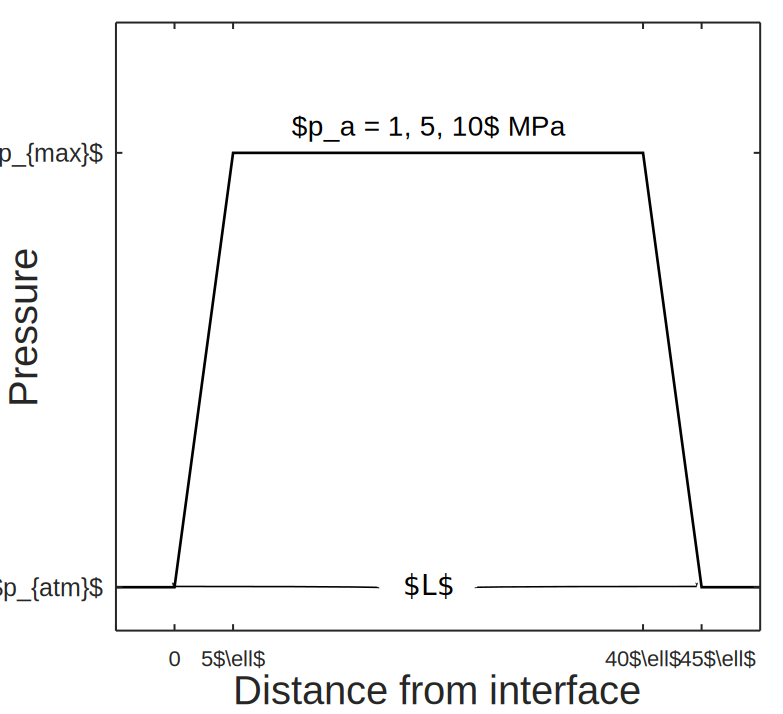
\includegraphics[width=0.5\textwidth]{./figs/lung_figs/p0_vs_y}
  \caption{Initial pressure in the domain as a function of distance from the interface.}
  \label{fig:p0_vs_y}
\end{figure}

We solve the dimensionless Euler equations of compressible, inviscid
fluid motion in two dimensions ($x,y$),
\begin{subequations} \label{eq:euler}
  \begin{align} 
    \frac{\partial \rho}{\partial t} + \frac{\partial \left(\rho u\right)}{\partial x} + \frac{\partial \left(\rho v\right)}{\partial y} = 0,\\
    \frac{\partial \rho u}{\partial t} + \frac{\partial}{\partial x}\left( \rho u^2+p\right)  + \frac{\partial}{\partial y}\left( \rho uv\right) = 0,\\
    \frac{\partial \rho v}{\partial t} + \frac{\partial}{\partial x}\left( \rho uv\right)  + \frac{\partial}{\partial y}\left( \rho v^2+p\right) = 0,\\
    \frac{\partial E}{\partial t} + \frac{\partial}{\partial x}\left[u\left(E+p\right)\right] + \frac{\partial}{\partial y}\left[v\left(E+p\right)\right] = 0,
  \end{align}
\end{subequations}
where $\rho$ is density, $p$ is the pressure, $u$ and $v$ are the
velocity components in the $x$ and $y$ directions respectively, and
$E$ is the total energy. We use the density and sound speed of air to
nondimensionalize the system. To close the system, we use a stiffened
equation of state which relate the total energy to the pressure and
velocity in the flow, such that,
\begin{align}\label{eq:stiffened_eos}
  E=\frac{\rho\left(u^2+v^2\right)}{2} + \frac{p+\gamma B}{\gamma-1}.
\end{align}
Here $B$ is a measure of liquid stiffness. For perfect gases, such as
is our treatment of air, $\gamma$ is the specific heats ratio and
$B=0$. It is worth noting that the sound speed in our simulations is
calculated based on the following relationship, derived from the
stiffened equation of state.
\begin{align}
  c = \sqrt{\frac{\gamma\left(p+B\right)}{\rho}}
\end{align}
While physical diffusion is not considered in this setup, numerical
diffusion does occur at fluid interfaces, creating a mixed region
between the two fluids. To use a single equation of state, a mass
fraction $Y$ is used to determine the material parameters
($\rho, \gamma, B, c$) of the mixed fluid such that $Y=1$ for pure
water and $Y=0$ for pure air. Details of this implementation are
explained by \cite{HenrydeFrahan2015} and additional mixture relations
for properties can be found in \cite{Ward2010}. The
dimensional and dimensionless values of each fluid property can be
found in tables \ref{tab:usbe_lung_dimensional_parameters} and
\ref{tab:usbe_lung_dimensionless_parameters} respectively.
% 
\begin{table}[htbp]%
  \begin{center}
    \caption{Dimensional properties of air and water used in simulations.}
    \label{tab:usbe_lung_dimensional_parameters}%
    \begin{tabularx}{0.75\textwidth}{| X | X | X | X | X |}
      \hline
      & Density, $\rho^*$ (kg/m$^3$) & $\gamma$ & $B^*$ (Pa)  & $c^*$ (m/s) ($p$=$1$ atm) \\ \hline
      Air   & 1.1765                        & 1.4      & 0         & 347.23     \\ \hline
      Water & 996                           & 5.5      & 492115000 & 1648.7     \\ \hline
      \multicolumn{5}{l}{\small $^*$ indicates dimensional parameter}
    \end{tabularx}
  \end{center}
\end{table}%
\begin{table}[htbp]%
  \begin{center}
    \caption{Dimensionless properties of air and water used in simulations.}
    \label{tab:usbe_lung_dimensionless_parameters}%
    \begin{tabularx}{0.75\textwidth}{| X | X | X | X | X |}
      \hline
      & Density, $\rho$ & $\gamma$ & $B$ & $c$ \\ \hline
      Air   & 1                          & 1.4      & 0         & 1          \\ \hline
      Water & 846.6                      & 5.5      & 3469.1    & 4.75       \\ \hline
      \multicolumn{5}{l}{\small Parameters are nondimensionalized by the density and sound speed of air. }
    \end{tabularx}
  \end{center}
\end{table}

To solve the governing equations, we implement a third-order accurate
\ac{DG} scheme in space and a fourth-order accurate, adaptive
Runge-Kutta method to march forward in time
\citep{HenrydeFrahan2015}. A Rusanov approximate Riemann solver is
used to compute the flux.  As previously stated, the computational
domain width (x-direction) is $\lambda$. The domain length
(y-direction) is 70$\lambda$. The grid resolution is 100 points per
$\lambda$ unless otherwise stated. To minimize artificial reflections,
inflow and outflow boundary conditions are used at the top and bottom
of the domain, and the geometric grid stretching was implemented in
the vertical direction for the top and bottom-most 10$\lambda$
segments of the grid. Periodic boundary conditions are implemented at
the left and right edges of the grid.


\section{Analysis} \label{sec:usbe_lung_analysis} To answer the
questions presented at the end of
section \label{sec:usbe_lung_introduction}, we perform analysis to
make some predictions about the vorticity and interface dynamics of
the system to be solved. The results of this analysis are later
compared to the results of our numerical results in section
\ref{sec:usbe_lung_results} and discussed.

\subsection{Vorticity generation order of magnitude analysis}
We perform an order of magnitude analysis on each term of the
vorticity generation equation for a 2D inviscid fluid
system, 
\begin{align} \label{eq:vorticity_euler}
  \frac{\partial \vec{\omega}}{\partial t}+\left(\vec{u}\cdot\nabla\right)\vec{\omega} =% 
  - \vec{\omega}\left(\nabla\cdot\vec{u}\right) + \frac{\nabla\rho\times\nabla p}{\rho^2}.%
\end{align}
Each of these terms represents a different physical mechanism by which
the vorticity in the system is changing, with the terms on the left
side of the equation representing changes in the existing vorticity
field and the terms on the right representing vorticity sources and
sinks. The first term on the left represents the total change of
vorticity at any given point in the flow field. The second term on the
left represents the advection of vorticity within the field. The first
term on the right describes stretching of vorticity due to
compressibility in the flow. And the last term on the right is the
baroclinic term which represents vorticity generated by the
misalignment of the pressure and density gradients in the flow. For
our setup, we expect this to be governed by the pressure gradient of
the acoustic wave and density gradient across the pertubed interface
at points where the two meet obliquely.

To perform the analysis, we specifically we consider the period in
which the incoming compression wave is encountering the interface. It
is assumed that the interface is static an undeformed from its
initial state.



As the above analysis suggests that circulation initially deposited by
the compression wave is predominantly baroclinically generated we
predict that circulation deposited will increase linearly with maximum
acoustic pressure $p_a$, i.e.,
$\Gamma \sim \frac{\nabla \rho\times\nabla p}{\rho^2}\sim p_a$.

To numerically verify this prediction, we start from the vorticity generation equation for a 2D compressible, inviscid fluid.
\begin{align} \label{eq:vorticity_euler}
  \frac{\partial \vec{\omega}}{\partial t}+\left(\vec{u}\cdot\nabla\right)\vec{\omega} =% 
  - \vec{\omega}\left(\nabla\cdot\vec{u}\right) + \frac{\nabla\rho\times\nabla p}{\rho^2}%
\end{align}

To determine the relative contributions to the half-domain circulation
at each point in time we break the equation down into its individual
component terms and integrate each over the right half domain. Doing
this we arrive at the following set of equations,

\begin{align}
  \left(\frac{d\Gamma}{dt}\right)_{total} = \left(\frac{d\Gamma}{dt}\right)_{compressible} + \left(\frac{d\Gamma}{dt}\right)_{baroclinic} - \left(\frac{d\Gamma}{dt}\right)_{advective},
\end{align}

where 

\begin{align}
  &\left(\frac{d\Gamma}{dt}\right)_{compressible} &=& -\int_{A_R} \vec{\omega}\left(\nabla\cdot\vec{u}\right) \, dA_R,&\\
  &\left(\frac{d\Gamma}{dt}\right)_{baroclinic} &=& +\int_{A_R} \frac{\nabla\rho\times\nabla p}{\rho^2}, dA_R,&\\
  &\left(\frac{d\Gamma}{dt}\right)_{advective} &=& +\int_{A_R} \left(\vec{u}\cdot\nabla\right)\vec{\omega} \, dA_R,&
\end{align}

If the interface deformation after the wave has left the domain is
entirely due to circulation, we expect from dimensional analysis that
the interface amplitude will grow according to
$a(t)/a_0 \sim \sqrt{\Gamma t}$.


\section{Results and discussion} \label{sec:usbe_lung_results} Figure
\ref{fig:trapz10_circ_interface} shows the early-time interface
amplitude and half-domain circulation histories for the 10 MPa
trapezoidal wave impinging on the water-air interface.

\begin{figure}[h] 
  \centering
  \includegraphics[width=0.48\textwidth]{./figs/lung_figs/trapz10_intf_schematic}
  \includegraphics[width=0.48\textwidth]{./figs/lung_figs/trapz10_circ_schematic}
  \caption{The interface amplitude (left) and circulation (right)
    histories corresponding to the $10$ MPa trapezoidal waves are shown
    for $t\leq25$. Indicated times, $t_{1-4}$, are the times at which
    different stages of the incoming pressure wave shown in Figure
    \ref{fig:p0_vs_y} first encounter the interface.}
  \label{fig:trapz10_circ_interface}
\end{figure}

Figure \ref{fig:trapz_circ_interface} shows the interface amplitude
and half-domain circulation histories for 0$\leq t\leq$ 500 as
functions of time for 1, 5, and 10 MPa amplitude trapezoidal
waves impinging on the interface. The interface amplitude is plotted
on logarithmically-scaled axes. 

\begin{figure}[h] 
  \centering
  \includegraphics[width=0.48\textwidth]{./figs/lung_figs/interface_multi-amp_early}
  \includegraphics[width=0.48\textwidth]{./figs/lung_figs/circulation_multi-amp_early}
  \caption{The interface amplitude (left) and circulation (right) histories corresponding to the $1$(blue), $5$(orange), and $10$(yellow) MPa trapezoidal waves are shown for $t\leq 25$. The circulation history is normalized by the acoustic amplitude of the incoming wave to illustrate that circulation deposition scales linearly with $p_a$ \hl{(Update plot for Rusinov solver results)} }
  \label{fig:trapz_circ_interface_early}
\end{figure}

\begin{figure}[h] 
  \centering
  \includegraphics[width=0.48\textwidth]{./figs/lung_figs/interface_multi-amp_loglog}
  \includegraphics[width=0.48\textwidth]{./figs/lung_figs/circulation_multi-amp2}
  \caption{The interface amplitude (left) and circulation (right) histories corresponding to the $5$(orange) and $10$(yellow) MPa trapezoidal waves are shown for $t\leq 500$. \hl{(Update plot for Rusinov solver results)}}
  \label{fig:trapz_circ_interface_loglog}
\end{figure}

\begin{figure}[h] 
  \centering
  \includegraphics[width=0.48\textwidth]{./figs/lung_figs/placeholder}
  \caption{The time derivative of each term of the circulation generation equation is shown.}
  \label{fig:trapz_ddt_circ}
\end{figure}


\subsection{To be added to discussion}
\textcolor{red}{ For typical acoustic waves, the pressure, velocity, and
  density return to ambient conditions after the passing of the
  wave. This implies that given a continuous acoustic waveform, the
  integral the pressure gradient of over the entirety of the waveform
  will be zero.  Hence if this wave interacts with a non-deforming
  interface, the net baroclinic circulation deposited will be zero
  \hl{(Must this be true if the wave itself is deforming during
    interaction with the interface? I think so)}. Hence for an acoustic
  wave to deposit net baroclinic circulation upon an interface, the
  interface itself must deform during interaction with the wave. This
  deformation alters the misalignment of the pressure and density
  gradients at the interface, allowing for positive and negative
  circulation deposited to not cancel out entirely. \hl{(Consider how
    well the pressure gradient argument works in higher dimensions than
    1. How does the direction of that pressure gradient change, relative
    to the density gradient in 2D, 3D?)}  Note that this is not the case
  for a shock wave, as the fluid need not return to ambient conditions
  after the waves passing.}


\section{Conclusions} \label{sec:usbe_lung_conclusions}

\section{Future Work} \label{sec:usbe_lung_future}
There are still many tasks and questions left to be investigated.

\begin{itemize}
\item Can we predict the amount of circulation deposited by a given wave?
\item How would alveolar walls change the dynamics (thin layer of water on the side)?
\item What is causing late time circulation growth?
\item Why is the the Roe flux solver generating less circulation than the Rusinov?
\end{itemize}

%%% Local Variables:
%%% mode: latex
%%% TeX-master: "../main"
%%% End:
